\documentclass[10pt,twocolumn]{article}

\usepackage{graphicx,url}
\usepackage{subfigure}

\usepackage[brazil]{babel}
\usepackage[utf8]{inputenc}
\usepackage{times}
\usepackage{subfigure}
\usepackage{graphicx}
\usepackage[pdftex,colorlinks,%
                   citecolor=black,%
                   filecolor=black,%
                   linkcolor=black]{hyperref}

%%%%%%%%%%%%%%%%%%%%%%%%%%%%%%%%%%% Header  %%%%%%%%%%%%%%%%%%%%%%%%%%%%%%%%%%%

\title{Recuperação de Informação \\Trabalho Prático 3 -- Processamento
de Consulta}
\author{Tiago Alves Macambira \\ \texttt{tmacam@dcc.ufmg.br}}
\date{29 de julho de 2007}

%%%%%%%%%%%%%%%%%%%%%%%%%%%%%%%%%%%  Body  %%%%%%%%%%%%%%%%%%%%%%%%%%%%%%%%%%%

\begin{document}
\maketitle

\section{Introdução}

O terceiro trabalho prático da disciplina de Recuperação de Informação
consiste no projeto e implementação de programas para
recuperação eficiente de grandes base de dados. Tal trabalho é uma
extensão do trabalho realizado no TP anterior, possuindo os seguintes
requisitos adicionais, como disposto no seu enunciado~\cite{tp3}:
\begin{itemize}
\item O sistema deve utilizar como base os dados coletados pelo
\emph{crawler} do TP1~\cite{tp1}.
\item Diferentemente do TP2, neste trabalho o aluno deverá processar e
\emph{rankear} consultas usando o modelo de espaço
vetorial~\cite{tp2}.
\item O sistema deve possuir uma interface \emph{Web} com a qual
o usuário interagirá com o mesmo.
\item Opcionalmente o sistema pode se utilizar de mecanismos de análise
de \emph{link} como forma de melhorar a qualidade da resposta gerada
pela solução.
\item O sistema deve ser escrito em C/C++. Bibliotecas extras somente
poderão ser utilizadas mediante autorização dos professores.
\end{itemize}

Nesse relatório, comentaremos sobre a resolução do nosso trabalho:
os desafios encontrados, as escolhas de projetos
adotadas e peculiaridades de nossa implementação. Além disso, comentamos
sobre o desempenho do mesmo, as estruturas de dados usadas bem como suas
complexidades.

Muitos dos pontos abordados nos trabalhos práticos anteriores são também
relevantes a esse trabalho prático. Por esse motivo e para tornar a
leitura desse relatório independente da leitura dos relatórios
anteriores, sempre que necessário, utilizaremos fragmentos dos mesmos.
Todavia, buscaremos não detalhar mais do que o necessário decisões
de projeto e peculiaridades dos TPs anteriores.

\vspace{0.5cm}
\rule[0.5mm]{0.9\linewidth}{0.5mm}

A implementação atual de nossa solução\
 se encontra operacional no
endereço \texttt{http://mimosa.grad.dcc.ufmg.br:8090}.

\rule[0.5mm]{0.9\linewidth}{0.5mm}


\section{Recuperação de documentos}\label{sec:retrieval}

Dado um conjunto de páginas \emph{Web} coletadas, para que seja possível
realizar buscas eficientemente nessa coleção é necessário, antes de mais
nada, indexar o seu conteúdo.

Uma vez que esse conteúdo tenha sido indexado, resta então o problema
de recuperar documentos da coleção que atendam uma ``necessidade de
informação'' ou consulta de um usuário. Ou seja, dada uma busca solicitada por um
usuário, representada através de um
conjunto de palavras-chaves (\emph{query}), localizar na colação
documentos que atendam a essa busca e, por alguma métrica, ordenar esses
documentos de forma a priorizar a exibição no topo dessa lista de
documentos mais relevantes. É importante frisar que
\emph{relevância} é uma prerrogativa do usuário. Tudo o que o sistema
pode fazer é se utilizar de heurísticas que priorizarão documentos que
\emph{devem}, sob a ótica do usuário, ser mais relevantes.

Uma das formas mais utilizadas atualmente por sistemas de buscas para
estimar a relevância de documentos dada uma consulta consiste no uso de
alguma medida de \emph{similaridade} entre os documentos e a consulta. A
intuição é que quanto maior a similaridade entre um dado documento e a
consulta, maior será a chance de que um humano considere esse documento
como relevante~\cite{moffat2006survey}.

Existem diferentes formas de determinar se um dado documento
atende (\emph{match}) uma busca  realizada pelo usuário e, associadas a
essas formas, diversos mecanismos de ordenação dos resultados. Cada uma
destas formas determina diferentes \emph{modelos de recuperação de
documentos}. No trabalho prático anterior implementou-se o modelo
booleano para recuperação de documentos. Neste, é solicitada a
implementação do modelo de espaço vetorial(\emph{Vector-Space Model}).

\subsection{Modelo de espaço vetorial}

No modelo de espaço vetorial tanto um documento \(D\) como uma busca
\(Q\) são representados como vetores em um espaço \(t\)-dimensional,
onde \(t\) é o número de termos no vocabulário da coleção. A
similaridade entre um documento e a busca é dada pela ângulo entre esses
dois vetores~\cite{berthier1999modern}.
Esse ângulo é obtido através do cálculo do cosseno entre
os vetores de \(D\) e \(Q\), apresentada na equação~\ref{eq:sim}:

\begin{equation}
Sim(d_{j},q) = \frac{\sum_{i = 1}^{t}w_{i,j} w_{i,q}}{\sqrt{\sum_{i =
1}^{t}w_{i,j}^{2}} \sqrt{\sum_{j = 1}^{t}w_{i,q}^{2}}}
\label{eq:sim}
\end{equation}

Observe que \(w_{i,j}\), o peso do termo \(i\) no documento \(j\), é
dado pela equação~\ref{eq:tfidf}:


\begin{equation}
w_{i,j} = tf_{i,j}\times idf_{i}
\label{eq:tfidf}
\end{equation}

As fórmulas de \(tf_{i,j}\), que representa o quanto um termo é
discriminante em um dado documento, e de \(idf_{i}\), que representa o
quanto um dado termo é discriminatório sob o ponto de vista da coleção
como um todo, são apresentadas nas equações~\ref{eq:tf} e~\ref{eq:idf}:

\begin{equation}
tf_{i,j} = \frac{freq_{i,j}}{max freq_{j}}
\label{eq:tf}
\end{equation}

\begin{equation}
idf_{i} = log\frac{N}{n_{i}}
\label{eq:idf}
\end{equation}

É importante observar que, dada uma consulta, a norma do seu vetor
(\(|Q|\)), pode ser omitida dos cálculos para fins de ordenação de
resultados, uma vez que nesse caso ela será constante.

\subsection{Análise de links}

Além da similaridade, outras informações, tais como
proximidade entre palavras-chaves, taxa de atualização dos documentos,
 quantidade de \emph{links} de saída ou de \emph{links} de chegada em uma página
etc, podem ser utilizadas no processo de \emph{ranking} de documentos.

O uso de informações sobre sobre a ligação de uma página com as outras
(seus \emph{links}), ou \emph{link analysis}, tem se mostrado bastante
satisfatório, não somente no contexto de \emph{ranking} de documentos
mas também em políticas de escalonamento de
\emph{crawling}~\cite{baezayates2005crawling}. Todavia, a forma de se
utilizar essa informação e de aferir a esta um valor pode variar
bastante. Na literatura encontramos propostas tais como o HITS e o
PageRank que diferem na forma como que a informação de \emph{links} de
uma página é utilizada~\cite{page98pagerank}.

No modelo do \emph{PageRank}, a cada página é atribuído um valor, que
representa, de certa forma, a ``importância'' dessa página tal como ela
é vista pela relação de \emph{links} da \emph{Web}. De outra forma, o
\emph{PageRank} de uma página pode ser visto como medindo a chance de
que um surfista aleatório atinja uma determinada página.

Sejam \(u\) uma página, \(PR(u)\) o valor do \emph{PageRank} da página
\(u\), \(B_u\) o conjunto de páginas que possuem
\emph{links} para \(u\) e \(N_v\) o número de \emph{links} que
partem de uma página qualquer \(u\) para outras páginas na coleção ou na
\emph{Web}. Assim sendo, o \emph{PageRank} pode ser definido da
seguinte:

\begin{equation}
 PR(u) = (1-d) + d\sum_{v \in B_u}\frac{PR(v)}{N_v}
\label{eq:pagerank}
\end{equation}

Essa fórmula é recursiva mas o calculo do \emph{PageRank} para alguns
milhões de páginas pode ser feito eficientemente em questão de horas
utilizando um algoritmo iterativo~\cite{brin1998google}.

%Nessa fórmula, \(d\)



\section{Problemas e desafios}

Nessa seção comentaremos sobre alguns dos problemas que podem ser
encontrados durante o processamento de consultas utilizando o modelo de
espaço vetorial e realizando análise de \emph{links} usando o PageRank.
seção~\ref{sec:implementation} comentaremos como lidamos com esses
problemas na nossa implementação.

\subsection{Escolha do modelo de TF-IDF}

Além das fórmulas apresentadas na seção~\ref{sec:retrieval}, existem
outras fórmulas para o cálculo de TF-IDF. Apesar da similaridade em
função de várias delas, é necessário observar que cada um possui
pequenas particularidades que podem torná-las mais atraentes para alguns
determinados tipos de documentos ou coleções mas não para os demais.

\subsection{Valores pré-computados}

Tanto o modelo de espaço vetorial como o PageRank assumem que alguns
valores estão pré-computados ou que sua obtenção é fácil. Entre tais
valores podemos citar a norma ou o módulo de vetores de cada documento,
o número de ocorrências do termo mais freqüente de cada documento e o valor de
PageRank de cada documento da coleção.

Obter esses valores em tempo de consulta é inviável. Alguns podem ser
calculados tão logo se termine a etapa de indexação dos
documentos, outros só poderão ser obtidos após o término da geração do
arquivo invertido. O momento e a forma de fazer isso pode ocasionar um
acréscimo de tempo de pré-processamento grande e, por isso, deve ser
dosado.

\subsection{Formas eficientes de calcular similaridade}

Apesar da diferença entre os modelos booleano e o modelo de espaço
vetorial, a forma de se realizar processamento de consulta em ambos os
modelos possui algumas similaridades. Uma das mais óbvias é o fato de
que ambas utilizam as listas invertidas dos termos presentes na coleção
(e apenas estes) para a realização da consulta.

No entanto, no modelo vetorial, para cada lista invertida será
necessário acrescentar o peso que o termo daquela lista invertida
acrescentará no valor de similaridade de cada um dos documentos
existentes. Dependendo do tamanho da lista invertida, isso pode se
tornar caro, especialmente no caso de \emph{stopwords}, que possuem
listas invertidas bem maiores à média.

Diversas estratégias podem ser adotadas para tornar esse cálculo mais
eficiente ou até mesmo para evitar que cálculo desnecessário tenha de
ser feito. Uma das abordagens mais simples é limitar as consultas apenas
a buscas conjuntivas, limitando assim a quantidade de acumuladores que
têm de ser armazenados na memória a cada interação. Outras abordagens
possíveis são o uso de listas de impacto ou na reordenação das
listas invertidas por valores de freqüência de
documentos~\cite{moffat1999managing, persin1996frequency}.

\subsection{Extração de \emph{Links}}

Para a realização de \emph{link analysis} é necessário a obtenção da
lista de \emph{links} existentes em um dado documento \emph{Web}.
Essa atividade é relizada durante o
\emph{crawling} dos documentos mas, caso essa informação não tenha sido
armazenada nesse momento, será necessário realizar novamente o
\emph{parsing} de todos os documentos. Sendo esse o caso, alguns dos
problemas que têm que ser enfrentados ao se realizar o \emph{parsing} de
documentos durante o \emph{crawling}, muitos destes mencionados no TP1 e no TP2, terão de ser
enfrentados novamente:
\begin{itemize}
\item Normalização de mapas de caracteres
\item Descoberta de mapa de caracteres
\item \emph{Parsing} de páginas HTML
\item \emph{Parsing} de entidades
\item Internacionalização e \emph{tokenização} de texto
\end{itemize}

\subsection{Lidar com páginas-sumidouros}

Página-sumidouros (\emph{sinks}) são páginas que não apresentam
\emph{links} de saída. Tais páginas além de penalizar o valor de
PageRank de outras páginas também tornam a convergência do cálculo do
PageRank mais lenta~\cite{haveliwala99efficient, page98pagerank}.

Decidir como, se e quando esse tipo de página será tratado é uma decisão
que o implementador deve tomar.

%%%%%%%%%%%%%%%%%%%%%%%%%%%%%%% PROJETO %%%%%%%%%%%%%%%%%%%%%%%%%%%%

\section{O projeto do processador de consultas}\label{sec:projeto}

Realizamos o projeto de nosso processador de consultas tendo em mente os desafios
mencionados na seção anterior e algumas decisões tomadas durante os
trabalhos práticos 1 e 2~\cite{tp1,tp2}. Algumas decisões de projeto tiveram que
ser tomadas tanto para contornar tais problemas como para ser capaz de
completar o trabalho em um prazo razoável.


\subsection{Premissas e decisões iniciais de projetos}

Como forma de limitar o volume de processamento realizado por consulta e
também como forma de melhorar os resultados das buscas submetidas ao
sistema, \textbf{processamos todas as buscas como buscas conjuntivas}.
Em nossos testes essa escolha apenas melhorou a qualidade das respostas.

\textbf{A obtenção das normas dos documentos (\(W_j\)) e dos
\(maxfreq_i\) será feita apenas após a construção do arquivo invertido}.
As normas apenas podem ser calculadas quando tivermos os valores de
\(n_i\), ou seja, número de documentos contendo um determinado termo
\(i\), e isso só é possível após o termino da criação do arquivo
invertido. Além disso, esse arquivo é consideravelmente menor do que a
coleção de documentos, e o processamento realizado para sua leitura bem
inferior ao do \emph{parsing} de documentos.

\textbf{A obtenção do grafo de vizinhança de páginas}, ou seja, da lista de
ligações entre documentos da nossa coleção, \textbf{ocorre após a coleta de
todas as páginas}. Caso fôssemos realizar o uma nova coleta de páginas,
repensaríamos esse ponto. Todavia, como o \emph{crawling} já foi feito, isso
realmente não representa muito uma decisão de projeto, mas apenas uma
forma viável de contornar essa limitação de nosso \emph{crawler}.


\textbf{Todas as URLs processadas pelo algoritmo de \emph{link analysis} são
normalizadas} e têm seus campos \emph{query} e fragmento removidos. Os
mecanismos de normalização são os mesmos descritos nos TPs anteriores,
ou seja, baseados nas especificações da RFC 3986~\cite{rfc3986}.

Para contornar o volume de memória necessário para o armazenamento e
processamento do grafo de vizinhança \textbf{utilizaremos não as URLs em si, mas
suas ``impressões digitais''} (\emph{fingerpring}, geradas pelo uso da
função ou \emph{hash} FNV-1~\cite{fnv1}. Observamos essa função \textbf{não
apresenta colisões mesmo para o conjunto de aproximadamente 9 milhões de
URLs descobertas pelo nosso \emph{crawler}}.

\textbf{Removemos \emph{dangling links}}, ou seja, \emph{links} para
páginas-sumidouros em dois momentos:
\begin{enumerate}
\item durante a re-leitura da base, quando fazemos a extração das URLs
dos documentos,
\item durante o cálculo do PageRank, quando removemos interativamente
\emph{links} para páginas que se mostraram como páginas sem ligações de 
saída (\emph{outlinks}).
\end{enumerate}

Devido ao tamanho de nossa base e às características de ligação dos
nossos documentos, \textbf{o processamento do \emph{PageRank} envolverá
memória secundária}. Não como armazenamento secundário, mas simplesmente
\textbf{pelo fato de que o grafo não cabe na memória primária}. Mais a
frente discutiremos isso e o desempenho dessa etapa.

\textbf{Assumimos que várias das nossas estruturas de controle caberão na
memória}. Entre tais estruturas temos:
\begin{itemize}
\item o vocabulário,
\item as normas dos documentos,
\item a freqüência do termo mais freqüente de cada documento,
\item o valor de PageRank de cada documento,
\item o índice da base de títulos de URLs dos documentos.
\end{itemize}

\textbf{A interface entre o nosso sistema e o usuário se dá através de um
servidor HTTP próprio, single-threaded e blocante}. Esse servidor foi
feito especificamente para esse projeto e, a despeito de suas
limitações, atende aos propósitos da disciplina.

\subsection{Componentes}


Os componentes da no nosso \emph{processador de consultas} são:
\begin{description}
\item[armazém de dados:] esse sistema foi decomposto em dois, um sendo 
uma fina camada sobre o sistema de arquivos que
permite organizar os dados coletados/indexados e outra sendo um base de
dados indexada para acesso sequencial (ISAM), que permite acesso
sequencial muito mais rápido do que o sistema anterior.
\item[mknorms:] realiza a leitura e processamento do arquivo invertido
para geração das normas dos documentos e de outros dados que são
utilizados durante o processamento de consultas.
\item[mkmeta:] realiza o \emph{parsing} dos documentos e extrai desses
seus títulos e suas URLs, para uso posterior.
\item[mkprepr:] realiza o \emph{parsing} dos documentos e extrai destes
a lista de ( \emph{fingerprints} de) URLs de saída (\emph{outlinks}) de
cada página. A saída desse componente é utilizada como entrada para o
programa que calcula o PageRank das páginas.
\item[myserver:] nossa interface com o processador de consultas, ou
seja, nosso servidor HTTP. O processador de consultas em si encontra-se
como um componente usado em por esse servidor.
\end{description}


%%%%%%%%%%%%%%%%%%%%%%%%%%%%%% IMPLEMENTAÇÃO %%%%%%%%%%%%%%%%%%%%%%%%

\section{Implementação}\label{sec:implementation}

\subsection{Decisões de implementações}

Todo o nosso código foi escrito em C++
e utiliza a biblioteca de gabaritos padrões (STL) dessa
linguagem~\cite{stroustrup97}.
Não foi utilizada nenhuma nova biblioteca em comparação às já utilizadas
no TP1.

Além disso, nosso código faz uso extensivo de uma técnica para controle
de recursos (como memória, \emph{locks} etc)  muito comum em C++,
denominada RAII (\emph{Resource Acquisition Is Initialization}).
Diversas partes de nosso código possuem código de teste (\emph{Unit
Testing}).

Sempre que possível, delegamos o processo de leitura de
arquivos ao S.O. através do uso de \texttt{mmaps}.

\subsection{Estruturas de armazenamento}\label{sec:storage}

A forma como que os dados são gravados e recuperados do disco é
tão importante quanto os algoritmos e estruturas de dados utilizados
pelo nosso indexador. As estruturas de armazenamento podem ditar ou
limitar a efetividade dos algoritmos utilizados.

Em nossa solução, a exceção dos arquivos coletados pelo crawler, todas
as outras estruturas (vocabulário, arquivo invertido, metadados sobre as
páginas, valores de PageRank) possuem uma estrutura
de armazenamento similar (ISAM) e composta, de maneira geral, de dois
elementos:
\begin{description}

\item[Arquivo-cabeçalho] Uma estrutura que permite acesso rápido a
informações sobre um determinado termo ou documento.  Tais informações
consistem, entre outras coisas, na localização (\emph{offset} ou
ponteiro) do conteúdo de interesse no arquivo(s) de dados . \footnote{
Na prática, esse arquivo nada mais é do que o \emph{dump} de um
\emph{array}, o que, ao utilizarmos técnicas como \texttt{mmap}, permite
o aceso quase que em tempo constante à informação desejada.}

\item[Arquivo(s) de dados] Nesse arquivo, termos do vocabulário ou listas
invertidas propriamente ditas são armazenadas concatenadas. A
localização de um item em um arquivo de dados depende da leitura do
arquivo-cabeçalho correspondente.
\end{description}

No caso do vocabulário, o arquivo de dados consiste na concatenação das
palavras do vocabulário em ordem ascendente de seus \(t_{id}\).

As listas invertidas podem, quando concatenadas, podem vir a atingir um tamanho
superior ao tamanho máximo de um arquivo no SO utilizado. Para evitar
problemas, os dados das listas invertidas e de outras estruturas de
dados grandes, são distribuídos entre vários
arquivos de dados, cada um de aproximadamente 256~MB. A localização de
uma lista invertida relativa a um termo em um destes arquivo de dados
bem como a informação de em qual arquivo de dados essa lista se encontra
é guardada no arquivo-cabeçalho do arquivo invertido. De maneira similar
é possível encontrar, por exemplo, a lista de \emph{outlinks} de uma
dada página.

\subsection{Estruturas de dados}\label{sec:datastructures}

Nossa implementação usa as seguintes estruturas de
dados~\cite{cormen-algorithms}:

\begin{itemize}

\item No processamento de consulta, se utiliza uma
\emph{hashtable} (termo\(\rightarrow t_{id}\)) para armazenar o
vocabulário.  Busca e inserção nessa estrutura possui uma complexidade
de tempo médio de \(O\left(1 \right)\). Uma \emph{hashtable} também é
utilizado no processo de cálculo do PageRank (nossos identificadores não
são seqüenciais) e, na coleta de página, para verificação se cada as
novas páginas descobertas pertencem ao conjunto de páginas que foram
efetivamente coletadas.

\item Nos vários pontos em que é necessário realizar ordenação dos dados
(geração do resultado do modelo de espaço vetorial, ordenação do
resultado do casamento do modelo vetorial com o PageRank, etc) utilizamos
o algoritmo \emph{introsort}\footnote{ D. R. Musser,
"Introspective Sorting and Selection Algorithms", Software Practice and
Experience 27(8):983, 1997.  } cuja complexidade de pior caso é
\(O\left(n \log n\right)\)

\item Na processamento da consulta no modelo de espaço vetorial a busca
conjuntiva é feita pela interseção duas-a-duas das listas de documentos
encontrados. Esse algoritmo possui custo liner.

\end{itemize}


\subsection{Dificuldades}

Nessa sub-seção discutiremos alguns dos problemas enfrentados durante a
elaboração e teste da nossa implementação.

\subsubsection{Obtenção das normas, etc}

Como mencionado anteriormente, um dos problemas que enfrentamos foi o
cálculo das normas dos documentos e de outros valores que são utilizados
pelo processador de consulta. Boa parte desse trabalho poderia ter sido
feito durante o TP1, que tratava da construção do arquivo invertido.

\subsubsection{Número de \emph{Links}}

Durante a elaboração do código responsável pelo cálculo do PageRank nos
defrontamos com o seguinte problema: nosso arquivo contendo a lista de
\emph{outlinks}, essencialmente uma representação do grafo de ligação
entre páginas como uma lista de adjacências, estava atingindo a marca de
aprox. 2,5~GB. Esse arquivo possuía apenas as \emph{fingerprints} de
cada URL, cada um ocupando 8 bytes. Mesmo considerando o
número de documentos baixados pelo \emph{crawler}, o número de
URLs descobertas pelo mesmo ( aprox. 1,5 milhões e 9 milhões) e número
médio de \emph{links} por páginas \emph{Web} como 11~\cite{page98pagerank}, ainda
assim verifica-se que o volume de 2,5 GB está muito longe do esperado.


\begin{figure}[ht]
\begin{center}
\includegraphics[width=0.5\textwidth]{plot_linkranking}
\end{center}
\caption{Distribuição de links por páginas. (Log-Normal)}
\label{fig:linkspp}
\end{figure}

Para determinar se existia alguma problema em nossa solução ou se
existia alguma anomalia dos dados coletados, verificamos como se dava a
distribuição de \emph{links} por página nos documentos de nossa coleção.
O resultado dessa análise pode ser visto na Figura~\ref{fig:linkspp}.
Nessa figura, disposta em escala log-normal, pode-se observar que existe
uma significativa proporção de nós que possui mais de 200 links de
saída. Isso explica o motivo pelo qual nosso arquivo de \emph{outlinks}
tornou-se tão grande.

Por amostragem determinou-se que boa parte desses links correspondiam a
páginas do sítio \texttt{letras.terra.com.br} e seus sub-domínios. Em
conjunto, existem 1019681 páginas em nossa base cujas URLs possuem o
fragmento de texto \texttt{letras.terra}. Isso corresponde a quase dois
terços de nossa base, o que explica ainda mais o que aconteceu: baixamos
muitas página desses sítio e esse sítio e seus subdomíno estão
fortemente ligados entre si.

Ao invés de retirar esses documentos da base para tornar o cálculo do
PageRank viável utilizando somente memória primária, decidimos por
realizar o cálculo do PageRank de tal forma que, a cada iteração, os
valores são re-lidos do disco.

\section{Determinação dos Pesos para o PageRank e para o Modelo de
Espaço Vetorial}

Outro problema enfrentado durante a elaboração do trabalho foi
determinar pesos para utilizar durante a combinação dos resultados do
PageRank com os resultados do modelo de espaço vetorial.

Antes de ter esses dois valores combinados, normalizamos cada um deles
pelo respectivo máximo valor retornado para uma dada busca e
determinamos a pontuação final de um \emph{match} \(i\) como mostrado na
equação~\ref{eq:combo}.

\begin{equation}
Score_i = c\times PageRank_i + (1-c)\times VectorSpace_i
\label{eq:combo}
\end{equation}

Nos nossos experimentos, determinamos que o melhor valor de \(c\) era de
\(0.6\). No entanto, é importante frisar que não realizamos testes
extensivos nesses valores e existe uma boa margem para possíveis ganhos
aí.


%%%%%%%%%%%%%%%%%%%%%%%%%%%%%%%%%%%%%%%%%%%%%%%%%%%%%%%%%%%%%%%%%%%%%%
\section{Testes e Resultados}

\subsection{Ambiente experimental}

Todos os testes de nossa implementação foram realizados em um micro do
laboratório de graduação do DCC/UFMG, rodando como S.O. Linux Gentoo
1.12.9, kernel 2.6.19-gentoo-r5, dotado de uma CPU Pentium 4 de
3.00~MHz, 1~GB de memória RAM e 1~GB de \emph{swap}.

\subsection{Resultados}

\begin{table}[htbp]
\centering
\begin{tabular}{|c|r|} \hline
Número de documentos			& 1.572.822		\\\hline
Volume do vocabulário			&	      29.948 KB \\\hline
Volume da base de dados 		&   			\\
          compactado 			&            43.460.994 KB \\
          compactado 			&   	  13.977.374 KB \\\hline
Volume das runs 			&	   7.180.092 KB \\\hline
Volume do índice  			&			\\
  sem compressão  			&	   5.764.740 KB \\
  com compressão  			&	   1.547.700 KB \\\hline
Tempo para geração das normas 		&	    7m59.778s	\\ \hline
Tempo para extração de \# links		&		4h12m02s \\ \hline
PageRank				& 		\\
Tempo para convergência& 02h51m21s	\\
Valor Residual (norma \(L_1\)		& 	0.0500221 \\
Nº de Iterações até covergência		& 	89	\\ \hline
Total de \emph{links} (arestas) válidas & 297.401.139	\\ \hline
  sem compressão 			&	   9m43.120s \\
  com compressão  			&	   7m12.012s \\\hline
Velocidade de indexação			&		\\
  doc/s		  			& 20,568		\\
  KB/s					& 562			\\\hline
Número de Termos			&     2.311.837	\\\hline
\hline
\end{tabular}
\caption{Dados sobre as coletas}
\label{tab:sumario}
\end{table}


A Tabela~\ref{tab:sumario} apresenta um sumário dos valores de
desempenho e de outras informações pertinentes sobre esse TP.

Observe que o tempo de geração de normas engloba também o 
tempo para a extração e geração de outros valores gerados pelo
utilitário \texttt{mknorms}, como \(maxfreq_j\) e \(n_i\). Observe ainda
que o total de arestas válidas corresponde apenas a ligações entre
páginas baixadas na coleção para páginas com URLs que correspondem a
páginas baixadas na coleção.

\subsubsection{Convergência do PageRank}

Mesmo realizando, a cada iteração, a leitura dos arquivos com as listar
invertidas, consideramos que nossa implementação do PageRank executou
com relativa velocidade. Cada iteração demora em média 115 segundos.

\begin{figure}[htb]
\begin{center}
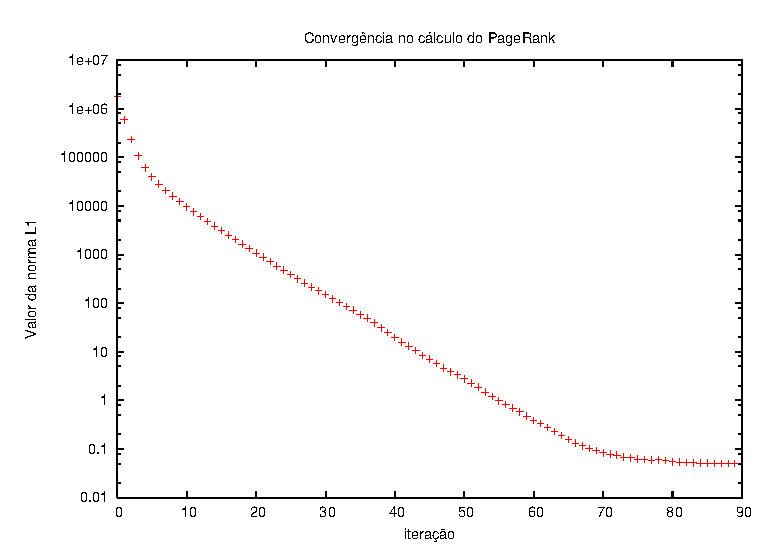
\includegraphics[width=0.5\textwidth]{plot_pagerankconverge}
\end{center}
\caption{Convergência do PageRank (escala Log-Normal)}
\label{fig:converge}
\end{figure}

Na Figura~\ref{fig:converge} podemos ver o gráfico de convergência do
PageRank, apresentado em escala Log-Normal. O valor da norma \(L_1\) é
calculado para as diferências das estimativas de PageRank encontradas em
duas execuções consecutivas. A fórmula para o cálculo da norma \(L_1\) é
apresentada na equação~\ref{eq:l1}. Como pode ser visto na figura, até
aproximadamente a interação 70 a curva apresenta o decaimento
exponencial -- evidenciado pela reta no gráfico em escala
log-normal. Após isso, o decaimento é consideravelmente mais lento,
indicando que para obter uma maior precisão (ou seja, um valor menor de
norma \(L_1\)), um número de iterações será bemm maior, não justificando
seu custo.

\begin{equation}
L_1(X) = \sum_{i=0}^{n}|x_i|
\label{eq:l1}
\end{equation}




%%%%%%%%%%%%%%%%%%%%%%%%%%%%%%%%%%%%%%%%%%%%%%%%%%%%%%%%%%%%%%%%%%%%%%
\section{Conclusões}


Nesse trabalho implementamos um processador de consultas utilizando o
modelo de espaço-vetorial e acrescentamos a ele um algoritmo de análise
de \emph{links}.

O que pudemos observar nos nosso experimentos é que, ao contrário do que
era de se esperar o uso de PageRank não melhorou as consultas. São duas
as hipóteses formuladas para explicar isso:
\begin{itemize}
\item má escolha da constante de combinação, como apresentada na
equação~\ref{eq:combo}.
\item algum problema inerente com a nossa base.
\end{itemize}

Esse último ponto merece destaque uma vez praticamente dois terços de
toda a coleção aparentam estar ligadas ao conteúdo e um único grande
sítio e conjunto de sub-domínios (\texttt{letras.terra.com.br}). Como
comentado mais acima, o conjunto de páginas desse grupo de domínios
possui características que nos levam a crer que elas possuem um grande
número de \emph{outlinks} e que estão fortemente ligadas. Desta forma, o
algoritmo do PageRank acabará por privilegiar essas páginas mais do que
quaisquer outras. Colocando de outra forma, nosso grafo não possui uma
amostra significativa da \emph{Web} na qual as características do
PageRank se sobressaem.


\section{Agradecimentos}

Esse trabalho não poderia ser entregue sem a ajuda de Hélio Almeida e
sem a colaboração de  Anísio Lacerda, que forneceu o código das funções
de hash.


%%%%%%%%%%%%%%%%%%%%%%%%%% Bibliografia %%%%%%%%%%%%%%%%%%%%%%%%%%%%%%

\bibliographystyle {plain}
\bibliography{relatorio}


\end{document}

% vim:tw=72 fileencoding=utf-8 spelllang=pt spell syn=tex:
